\iffalse
\documentclass[journal,10pt,twocolumn]{article}
\usepackage[margin=0.5in]{geometry}
\usepackage[cmex10]{amsmath}
\usepackage{array}
\usepackage{booktabs}

% The preceding line is only needed to identify funding in the first footnote. If that is unneeded, please comment it out.
\usepackage{cite}
\usepackage{amsmath,amssymb,amsfonts}
\usepackage{graphicx}
\usepackage{textcomp}
\usepackage{xcolor}
\usepackage{graphicx}
\graphicspath{{./figs}}{}
\def\BibTeX{{\rm B\kern-.05em{\sc i\kern-.025em b}\kern-.08em
    T\kern-.1667em\lower.7ex\hbox{E}\kern-.125emX}}

\usepackage{tikz}
\usetikzlibrary{shapes.geometric}
\usetikzlibrary{shapes.geometric,angles,quotes}


\begin{document}



\newtheorem{theorem}{Theorem}[section]
\newtheorem{problem}{Problem}
\newtheorem{proposition}{Proposition}[section]
\newtheorem{lemma}{Lemma}[section]
\newtheorem{corollary}[theorem]{Corollary}
\newtheorem{example}{Example}[section]
\newtheorem{definition}[problem]{Definition}
%\newtheorem{thm}{Theorem}[section] 
%\newtheorem{defn}[thm]{Definition}
%\newtheorem{algorithm}{Algorithm}[section]
%\newtheorem{cor}{Corollary}
\newcommand{\BEQA}{\begin{eqnarray}}
\newcommand{\EEQA}{\end{eqnarray}}
\newcommand{\define}{\stackrel{\triangle}{=}}
\newcommand*\circled[1]{\tikz[baseline=(char.base)]{
    \node[shape=circle,draw,inner sep=2pt] (char) {#1};}}

\bibliographystyle{article}
%\bibliographystyle{ieeetr}


\providecommand{\mbf}{\mathbf}
\providecommand{\pr}[1]{\ensuremath{\Pr\left(#1\right)}}
\providecommand{\re}[1]{\ensuremath{\text{Re}\left(#1\right)}}
\providecommand{\im}[1]{\ensuremath{\text{Im}\left(#1\right)}}
\providecommand{\qfunc}[1]{\ensuremath{Q\left(#1\right)}}
\providecommand{\sbrak}[1]{\ensuremath{{}\left[#1\right]}}
\providecommand{\lsbrak}[1]{\ensuremath{{}\left[#1\right.}}
\providecommand{\rsbrak}[1]{\ensuremath{{}\left.#1\right]}}
\providecommand{\brak}[1]{\ensuremath{\left(#1\right)}}
\providecommand{\lbrak}[1]{\ensuremath{\left(#1\right.}}
\providecommand{\rbrak}[1]{\ensuremath{\left.#1\right)}}
\providecommand{\cbrak}[1]{\ensuremath{\left\{#1\right\}}}
\providecommand{\lcbrak}[1]{\ensuremath{\left\{#1\right.}}
\providecommand{\rcbrak}[1]{\ensuremath{\left.#1\right\}}}

\newcommand{\sgn}{\mathop{\mathrm{sgn}}}

%\providecommand{\hilbert}{\overset{\mathcal{H}}{ \rightleftharpoons}}
\providecommand{\system}{\overset{\mathcal{H}}{ \longleftrightarrow}}
	%\newcommand{\solution}[2]{\textbf{Solution:}{#1}}
\newcommand{\solution}{\noindent \textbf{Solution: }}
\newcommand{\cosec}{\,\text{cosec}\,}
\providecommand{\dec}[2]{\ensuremath{\overset{#1}{\underset{#2}{\gtrless}}}}
\newcommand{\myvec}[1]{\ensuremath{\begin{pmatrix}#1\end{pmatrix}}}
\newcommand{\mydet}[1]{\ensuremath{\begin{vmatrix}#1\end{vmatrix}}}
	\newcommand*{\permcomb}[4][0mu]{{{}^{#3}\mkern#1#2_{#4}}}
\newcommand*{\perm}[1][-3mu]{\permcomb[#1]{P}}
\newcommand*{\comb}[1][-1mu]{\permcomb[#1]{C}}

%\numberwithin{equation}{section}
\numberwithin{equation}{subsection}
%\numberwithin{problem}{section}
%\numberwithin{definition}{section}

\let\vec\mathbf


\title{
{Quadrilateral with angles \\
Using lines}\\
}
\author{Suresh Beere}
\maketitle
\tableofcontents
\section{Problem statement}
\fi
The angles of quadrilateral are in the ratio 3:5:9:13. Find all the angles of the quadrilateral.
\iffalse

\section{Considerations}
\vspace{0.2cm}
\begin{flushleft}
As per given data, the following table has been prepared.\\
\end{flushleft}
\vspace{0.3cm}
\begin{table}[htbp]
    \centering
\setlength\extrarowheight{2pt}
\begin{tabular}{|c|c|c|} \hline
      \textbf{Symbol}           &   \textbf{Value}   & \textbf{Description}\\ \hline
	x &  & constant\\  \hline
	a & 3x & Angle A\\ \hline
	b & 5x & Angle B\\ \hline
    c & 9x & Angle C \\ \hline
    d & 13x & Angle D \\ \hline
\end{tabular}
\caption{\label{tab:widgets}Considerations}
\end{table}

\section{Plot of Quadrilateral}
\vspace{0.25cm}
Plot of the quadrilateral is shown in the figure 1.
\begin{figure}[h]
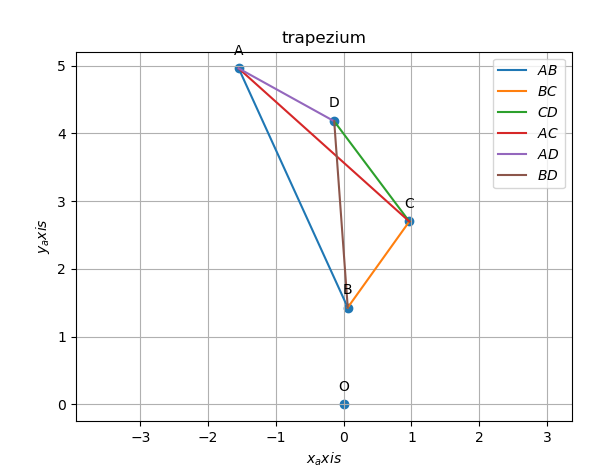
\includegraphics[width=1\columnwidth]{line.png}
\caption{Plot of Quadrilateral}
\end{figure}

\section{Solution}
\begin{flushleft}


Let angle in the ratio 3:5:9:13 be a,b,c,d\\
\vspace{0.25cm}
Let a=3x,b=5x,,c=9x,d=13x\\
\vspace{0.25cm}
where x is any number\\
\vspace{0.25cm}
We know that\\
\vspace{0.25cm}
Sum of angle of quadrilateral is 360\textdegree\\
\vspace{0.25cm}
a+b+c+d=360$\textdegree$   [Angle sum property of quadrilateral]\\
\vspace{0.25cm}
3x+5x+9x+13x=360\textdegree \\
\vspace{0.25cm}
30x=360\textdegree\\
\vspace{0.25cm}
x=360/30\\
\vspace{0.25cm}
x=12$\textdegree$\\
\vspace{0.25cm}
Hence the angles of Quadrilateral are\\
\vspace{0.25cm}
a=3x=3×12=36\textdegree\\
\vspace{0.25cm}
b=5x=5×12=60\textdegree\\
\vspace{0.25cm}
c=9x=9×12=108\textdegree\\
\vspace{0.25cm}
d=13x=13×12=156\textdegree
\end{flushleft}




\section{Software}
\begin{flushleft}
Download the codes given in the link below and execute them.\\
\end{flushleft}

\begin{table}[h]
\centering
\begin{tabular}{|c|} \hline
\rule{0pt}{10pt} 
https://github.com/sureshoye/line-assignment/blob \\
/main/codes/line.py\\
\\\hline
 \end{tabular}
\end{table}




\section{Conclusion}
\begin{flushleft}
The angles of Quadrilateral are\\
\vspace{0.25cm}
a=3x=3×12=36\textdegree\\
\vspace{0.25cm}
b=5x=5×12=60\textdegree\\
\vspace{0.25cm}
c=9x=9×12=108\textdegree\\
\vspace{0.25cm}
d=13x=13×12=156\textdegree
\end{flushleft}
\endcenter
\end{document}
\fi
